\documentclass[a0paper,portrait, 3pt]{baposter}

\usepackage{lipsum}          % This is just for some blindtext
\usepackage{biblatex}
\usepackage{relsize}	       % For \smaller
\usepackage{url}			       % For \url
\usepackage{epstopdf}	       % Included EPS files automatically converted to PDF to include with pdflatex
\usepackage{multicol}        % Multi Columns
\usepackage{graphicx}
\usepackage{float}
\usepackage{amsmath} % math
\usepackage{amssymb}
\usepackage{accents}
\usepackage[slovak]{babel}
\usepackage{csquotes}
\usepackage{xcolor}
\usepackage{marvosym}


%%%%%%%%%%%%%%%%%%%%%%%%%%%%%%%%%%%%%%%%%%%%%%%%%%%%%%%%%%%%%%%%%%%%%%%%%%%%%%%%
%%% Utility functions %%%%%%%%%%%%%%%%%%%%%%%%%%%%%%%%%%%%%%%%%%%%%%%%%%%%%%%%%%
%%%%%%%%%%%%%%%%%%%%%%%%%%%%%%%%%%%%%%%%%%%%%%%%%%%%%%%%%%%%%%%%%%%%%%%%%%%%%%%%

%%% Save space in lists. Use this after the opening of the list %%%%%%%%%%%%%%%%
\renewcommand{\vec}[1]{\bm{#1}}
%\renewcommand{\dot}[1]{\accentset{\cdot}{#1}}
\renewcommand{\ddot}[1]{\stackrel{..}{#1}}
%\newcommand{\tildeI}[1]{\overset{\tilde{}}{#1}} 

%\renewcommand{\bibname}{}

\newcommand{\vnabla}{\vec{\nabla}}

\renewcommand{\d}[1]{\text{d} #1}
\newcommand{\dxx}{\,\text{d}\vec{x}}
\newcommand{\dx}{\,\text{d}x}

\newcommand{\diff}[2]{\frac{\text{d}#1}{\text{d}#2}}
\newcommand{\idiff}[2]{\text{d}#1 / \text{d}#2}
\newcommand{\pdiff}[2]{\frac{\partial #1}{\partial #2}}
\newcommand{\pdifff}[2]{\frac{\partial^2 #1}{\partial #2^2}}
\newcommand{\ipdiff}[2]{\partial #1 / \partial #2}
\newcommand{\vdiff}[2]{\frac{\delta #1}{\delta #2}}
\newcommand{\ivdiff}[2]{\delta #1 / \delta #2}

\definecolor{mcr_purple}{RGB}{108,44,145}

%%%%%%%%%%%%%%%%%%%%%%%%%%%%%%%%%%%%%%%%%%%%%%%%%%%%%%%%%%%%%%%%%%%%%%%%%%%%%%%
%%% Document Start %%%%%%%%%%%%%%%%%%%%%%%%%%%%%%%%%%%%%%%%%%%%%%%%%%%%%%%%%%%%
%%%%%%%%%%%%%%%%%%%%%%%%%%%%%%%%%%%%%%%%%%%%%%%%%%%%%%%%%%%%%%%%%%%%%%%%%%%%%%%

\begin{document}
\typeout{Poster rendering started}

%%% General Poster Settings %%%%%%%%%%%%%%%%%%%%%%%%%%%%%%%%%%%%%%%%%%%%%%%%%%%
%%%%%% Eye Catcher, Title, Authors and University Images %%%%%%%%%%%%%%%%%%%%%%
\begin{poster}{
  columns=2,
	grid=false,
	borderColor=uniblue,
	headerColorOne=uniblue,
	headerColorTwo=uniblue,
	headerFontColor=white,
  headerheight=14em,
	boxColorOne=white,
  boxpadding=1em,
	headershape=rounded,
	headerfont=\Large\textsf,
	textborder=rounded,
	background=shadetb,
  bgColorOne=uniblue!10,
  bgColorTwo=uniblue!30,
	headerborder=open,
  boxshade=plain,
  eyecatcher=false
}
%%% Eye Cacther %%%%%%%%%%%%%%%%%%%%%%%%%%%%%%%%%%%%%%%%%%%%%%%%%%%%%%%%%%%%%%%
{ %\vspace{1em}
}
%%% Title %%%%%%%%%%%%%%%%%%%%%%%%%%%%%%%%%%%%%%%%%%%%%%%%%%%%%%%%%%%%%%%%%%%%%
{\vspace{1.25em} 
\smaller How long does it take for a cup of coffee to cool down?}
%%% Authors %%%%%%%%%%%%%%%%%%%%%%%%%%%%%%%%%%%%%%%%%%%%%%%%%%%%%%%%%%%%%%%%%%%
{
  \vspace{1.5em}
  {  \textbf{General Physics Group 55} \\
	{\smaller Diyaco Shwany, Jakub \v{S}\v{t}avina, Tomas Kvietkauskas, Phartav Murukutla, Aidan Hall, Jac Evans \\ 
    \textcolor{mcr_purple}{\smaller Department of Physics and Astronomy, University of Manchester}
    }
}
}
%%% Logo %%%%%%%%%%%%%%%%%%%%%%%%%%%%%%%%%%%%%%%%%%%%%%%%%%%%%%%%%%%%%%%%%%%%%%
{\begin{minipage}{18.0em}
    
\includegraphics[height=7.5em]{logo-uni.pdf}
  \end{minipage}}

%%% Abstract %%%%%%%%%%%%%%%%%%%%%%%%%%%%%%%%%%%%%%%%%%%%%%%%%%%%%%%%%%%%%%%%%%
\headerbox{Abstract}{name=abstract,column=0,row=0,span=2}{
%\begin{multicols}{2} 
We developed models for a cup of coffee utilising Newton's law of cooling and the heat equation to predict a timescale of cooling. The heat equation predicted that the coffee would cool down to 310 K in 52 minutes whereas the data suggests it should take 34 minutes. Finally, we investigated thermal convection within the coffee using the Lattice Boltzmann Method (LBM) to solve Navier-Stokes equations.

%\end{multicols}
}

%%% Box 1 %%%%%%%%%%%%%%%%%%%%%%%%%%%%%%%%%%%%%%%%%%%%%%%%%%%%%%%%%%%%%%%%%%%%%
\headerbox{Introduction}{name=box1,column=0,below=abstract%,above=bottom
}{As physics students, we often find ourselves in dire need of a productivity boost in the form of a cup of coffee. However, as most time is spent on physics, it is easy to be too eager to drink the coffee too soon or forget it so it goes cold. We aim to provide struggling students with an understanding of the temperature depenence on time of a cup of coffee left at room temperature.
%First, we performed a simple experiment and fit an empirical model based on Newton's law of cooling. To understand the underlying physics better, we then constructed a theoretical model of the heat equation on a rectangular cup of coffee.
 
  %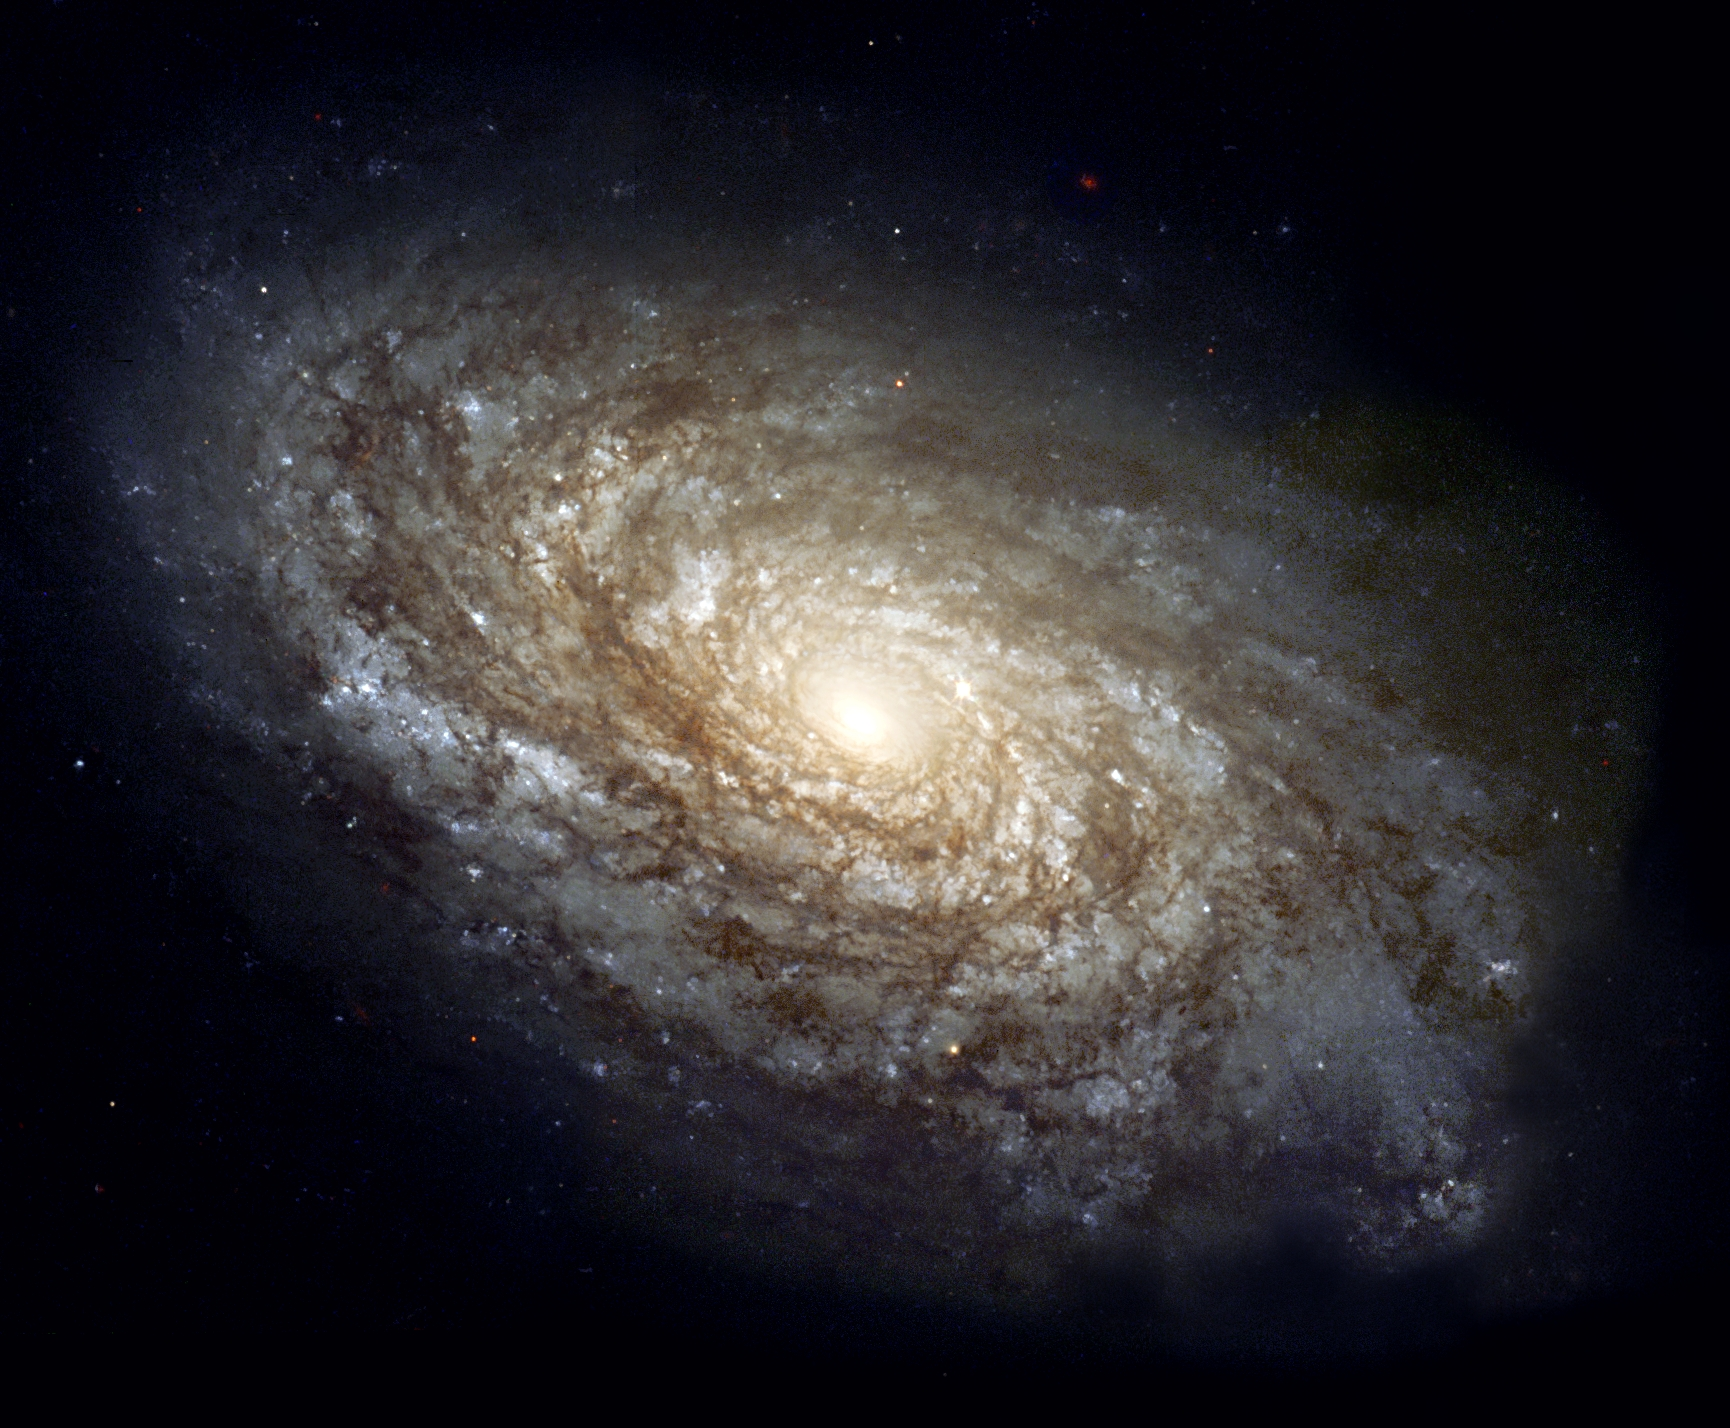
\includegraphics[width=\textwidth]{figure_1.jpg}
  %\caption{This is my caption.}
}

\headerbox{Theory}{name=model_0,column=0,below=box1%,above=bottom
}{Newton's law of cooling was the primary inspiration for the results that follow. This assumes that convection is the dominant form of cooling due to the surrounding air. The empirical model assumes the coffee to be a lumped capacitance object. This was developed through the heat equation which treats the coffee as a grid. Finally, convection within the coffee was explored by solving the 2D Navier-Stokes equation with the aid of lattice Boltzmann techniques. 
}

%%%%%%%%%%%%%%%%%%%%%%%%%%%%%%%%%%%%%%%%%%%%%%%%%%%%%%%%

\headerbox{Data and Empirical Model}{name=model_1,column=0,below=model_0%,above=bottom
}{Using a digital probe thermometer, we measured the temperature of a cup of hot coffee over time, as shown in Figure ?, at room temperature of 17°C. The starting temperature of the coffee ranged between 85 - 90°C.

Using Newton's law of cooling,

\begin{equation}
    \frac{dQ_{coffee}}{dt} = h_{air}A_{top}(T_{surr} - T_{coffee}) + h_{cup}A_{inner}(T_{cup} - T_{coffee})
\end{equation}
    
\begin{equation}
    \frac{dQ_{cup}}{dt} = h_{air} A_{outer}(T_{surroundings} - T_{cup}) + h_{cup}A_{inner}(T_{coffee} - T_{cup})
\end{equation}
assuming the transfer coefficient from the cup to the air is the same as that from the coffee to the air. Here the values $h_{air}$ and $h_{cup}$ are left to be determined empirically. The forward Euler method was applied to solve the equations. 

The model was then fitted to the experimental data, as shown in Figure ?. This yielded the values of the heat transfer coefficients of $h_{air} \approx 27.8$ $ Wm^{-2}K^{-1}$, $h_{cup} \approx 26.3 $ $Wm^{-2}K^{-1}$.

}


%%% Box 2 %%%%%%%%%%%%%%%%%%%%%%%%%%%%%%%%%%%%%%%%%%%%%%%%%%%%%%%%%%%%%%%%%%%%%
\headerbox{Theoretical Model}{name=model_2,column=1,below=abstract%,above=bottom
}
{

 The convective cooling was incorporated into the system as boundary conditions. To simplify calculations, we assumed the cup was a cuboid.
 
 We utilised the 3D heat equation as follows, 

\begin{equation}
    \frac{\partial T }{\partial t} = \alpha \left( \frac{\partial^2 T }{\partial x^2} + \frac{\partial^2 T }{\partial y^2} + \frac{\partial^2 T }{\partial z^2} \right)
\end{equation}

using the following robin boundary conditions, 

\begin{equation}
    \frac{\partial T}{\partial z} \Bigr|_{z = 0} = - \frac{h_{cup}}{k_{water}} (T - T_{\infty})
\end{equation}

\begin{equation}
    \frac{\partial T}{\partial z} \Bigr|_{z = H} = - \frac{h_{air}}{k_{water}} (T - T_{\infty})
\end{equation}

where $H$ is the height of the cup and $k_{water}$ is the thermal conductivity of water. The conditions in other coordinates were identical but all featured $h_{cup}$, as only the top of the cup is exposed to air. The empirical model values for $h_{cup}$ and $h_{air}$ were used.

The solution method was an explicit FDM scheme which discretised the system. The forward Euler scheme was used to integrate the boundary conditions across the outer walls. \\
The temperature against time plot was found by averaging the inner node contributions. However, this plot abstracts the temperature distribution which never fully became uniform in the simulation.
% 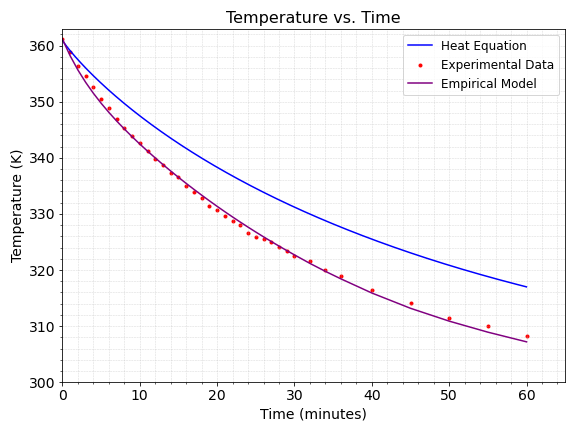
\includegraphics[width=\textwidth, scale=0.02]{Coffee-main/Coffee/Poster General Physics Project/temperature_plot__.png}

% \begin{figure}[H]
\begin{center}
    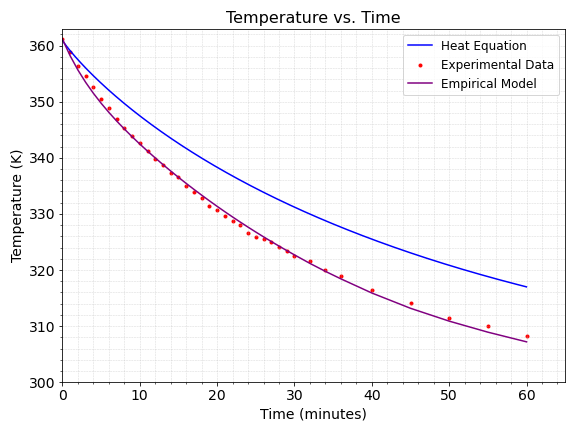
\includegraphics[scale=0.32]{Coffee-main/Coffee/Poster General Physics Project/temperature_plot__.png}
    
    % \caption{My Figure}
\end{center}
% \caption{This is my caption.}
% \end{figure}
}
\headerbox{Discussion}{name=conclusions,column=1,below=model_2}{  


The theoretical model incorrectly predicts that the coffee cools over a longer time period. Ignoring both evaporative cooling and convective mixing within the coffee contributed to the result. Evaporative cooling would cool , but its effect would diminish as the coffee cools down. The convective mixing would accelerate the heat dispersion within the coffee and homogenise it within a realistic time scale. Finally, our results from the Navier-Stokes equations form the basis for incorporating convective mixing. In future work, we plan on extending the lattice boltzmann technique to 3D and incorporate convective boundary conditions.



}


\headerbox{Lattice Boltzmann Method}
{name=model_3,column=0,below=model_1}{ 
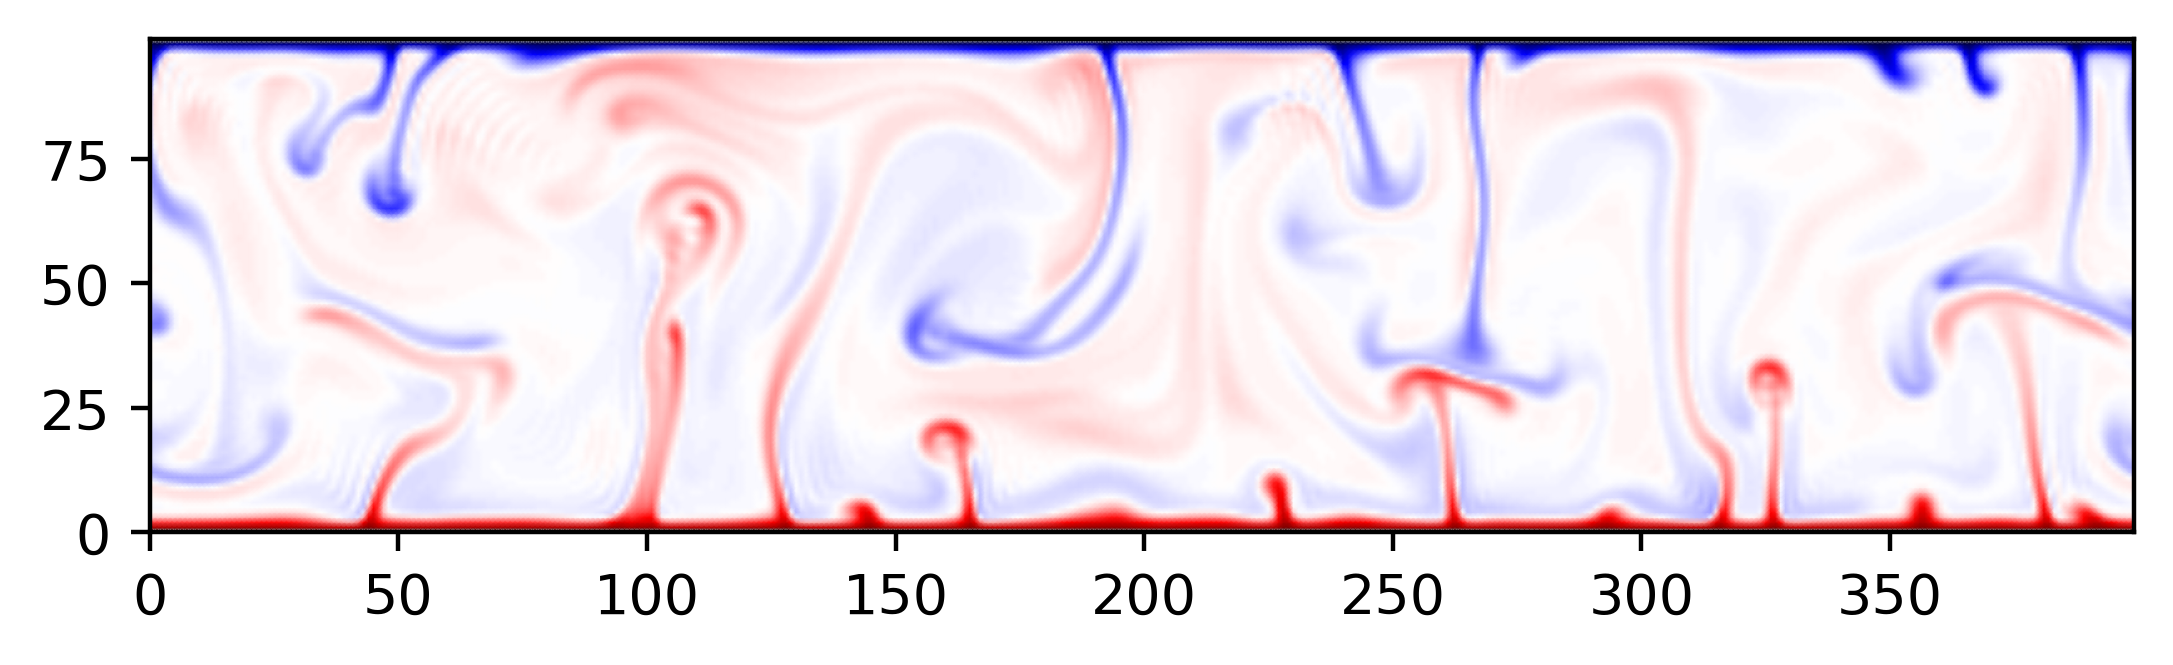
\includegraphics[width=\textwidth]{Coffee-main/Coffee/Poster General Physics Project/Temperature.png}

\begin{figure}[t]
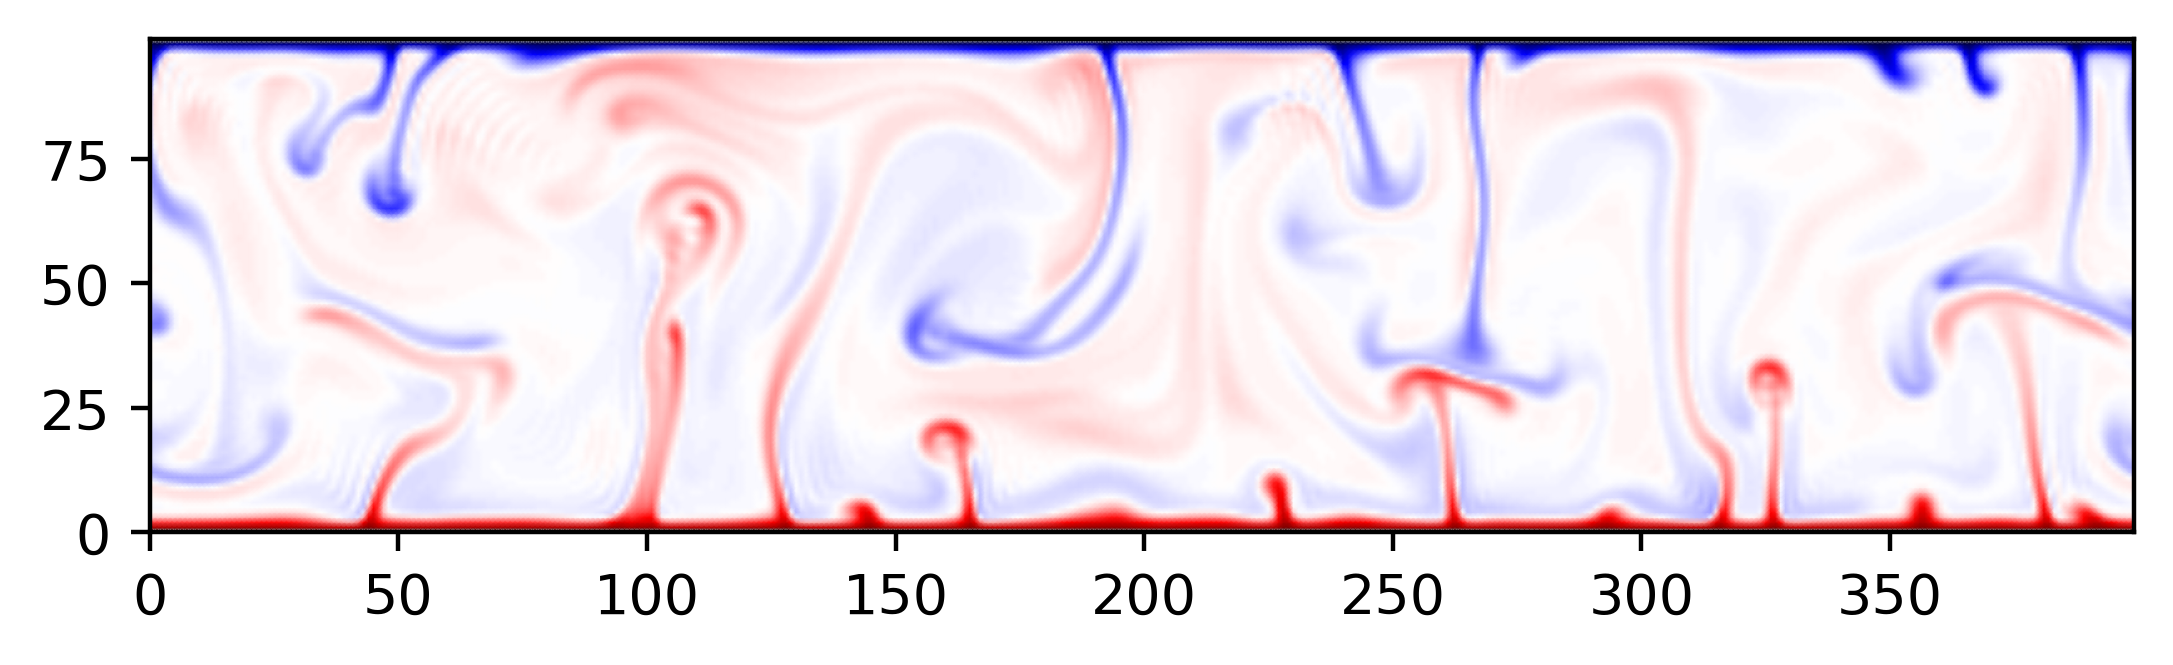
\includegraphics[width=0.5\textwidth]{Coffee-main/Coffee/Poster General Physics Project/Temperature.png}
\caption{This is my caption.}
\end{figure}

}


\headerbox{References}{name=references,column=0,below=model_3, span=2}{

\renewcommand{\section}[2]{}
\begin{thebibliography}{9}
\bibitem{Topinka2001} M. A. Topinka, B. J. LeRoy, R. M. Westervelt, S. E. J. Shaw, R. Fleischmann, E. J. Heller, K. D. Maranowski, and A. C.
Gossard, Nature (London) {\bf 410}, 183 (2001).
\bibitem{Patsyk2020} A. Patsyk, U. Sivan, M. Segev, and M. A. Bandres, Nature
(London) {\bf 583}, 60 (2020).
\bibitem{Kaplan2002} L. Kaplan, Phys. Rev. Lett. {\bf 89}, 184103 (2002).
\end{thebibliography}

}

\end{poster}
\end{document}

